\chapter{Research Proposal}
\label{ch:proposal}

This document previously demonstrated the performance of machine learning on a
set of nuclear material isotopics to calculate a reactor parameter of interest:
burnup.  Additionally, there have been various methods discussed for
understanding the learned model's behavior and thus the quality of the results.
Moving forward to a set of experiments is now possible.

Before describing the experiments, some topics and issues are addressed in
Section \ref{sec:prep}.  Finally, the proposed research experimental design is
presented Sections \ref{sec:exp1}, \ref{sec:exp2}, and \ref{sec:exp3}.

\section{Experiment Preparations}
\label{sec:prep}

\subsection*{Expanding Training Set}

As identified in Section \ref{sec:valid}, the testing set used for the
demonstration was not suitable for further study without being expanded.  Many
algorithms are developed on an assumption that the training set will be
\gls{i.i.d.}.  This is important so that the model does not overvalue or
overfit a certain area in the training space.  The next step is to provide a
larger, more diverse training set to the algorithms so they can better predict
when faced with new instances. This diversity will be suggested from the
\gls{SFCOMPO} database \cite{sfcompo}, as it includes many common domestic and 
international reactors.

The SFCOMPO-2.0 relational database \cite{sfcompo} has approximately 750
\gls{SNF} measurements from 44 reactors. While this is not sufficient as a
training set, it provides a better framework for simulating a larger training
set using \gls{ORIGEN}.  After cross-validation, diagnostics, and optimization,
the trained models can be tested against the entries in this database to
provide a clear estimate of of the model performance. 

\subsection*{Finalizing Set of Algorithms}

The three algorithms in the demonstration (nearest neighbor, ridge, and support
vector regression) are not necessarily the set that will be evaluated for the
experiments. After these are used to train new models on a larger training set
for comparison, other algorithms can be speedily evaluated as well.  Since
support vector-, distance-, and linear-based models are already represented,
other obvious choices include Bayesian methods, decision trees, neural
networks, or ensemble methods. 
\todo{mention in litrev or exclude....or cite book chapter}

\subsection*{Computational Framework and Resources}

Thus far, all simulations and training have not required more processing than
available on a personal laptop. However, some algorithms do require larger
amounts of computational time (e.g., artifical neural networks).  If necessary,
the training stage can be done using the \gls{CHTC}, which is available to
\gls{UW} researchers. 

\section[Experiment 1: Direct Isotopics]{Experiment 1\\ \large{\textit{Viability of Statistical Learning on Direct Isotopics}}}
\label{sec:exp1}

The first experiment will be a purposefully constructed version of the 
demonstration: evaluating the model performance  

Figure \ref{fig:proposal} blah blah

\begin{figure}[!htb]
    \centering
    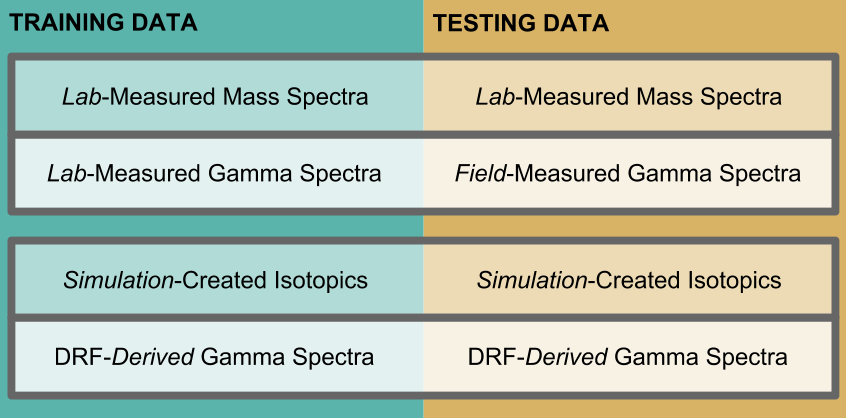
\includegraphics[width=\linewidth]{./chapters/proposal/proposal.png}
    \caption{Basis for Experiments 1 and 2.}
    \label{fig:proposal}
\end{figure}


\section[Experiment 2: Gamma Spectra]{Experiment 2\\ \large{\textit{Viability of Statistical Learning on Gamma Spectra}}}
\label{sec:exp2}

hey

hey

\section[Experiment 3: Other Fuel Cycle Flows]{Experiment 3\\ \large{\textit{Viability of Statistical Learning on Other Fuel Cycle Flows}}}
\label{sec:exp3}

hey 

hey
